 \documentclass[12 pt]{book}
\usepackage{amsmath}
\usepackage{amsthm}
\usepackage[paperwidth=5 in,paperheight=5 in,left=9 mm, right=9 mm, top=15 mm, bottom=18.5 mm]{geometry}
\usepackage{graphics}
\usepackage{fontawesome}
\usepackage{enumitem}
\usepackage{marvosym}
\newcommand{\myitem}{\refstepcounter{enumi}\item[$^\star$\theenumi.]}
\newcommand{\mmyitem}{\refstepcounter{enumi}\item[$^{\star \star}$\theenumi.]}
\setcounter{page}{01}

\usepackage[utf8]{inputenc}
\usepackage{xcolor}
\setlength{\arrayrulewidth}{0.1 mm}
%BLUE%
%\definecolor{Mycolor2}{HTML}{3D9BE9}
\definecolor{Mycolor2}{HTML}{33cccc}
%\definecolor{Mycolor2}{HTML}{000000}

%%----HEADER &&& FOOTER----%%

\usepackage{fancyhdr}


\pagestyle{fancy}
\fancyhf{}
\setlength{\headheight}{8 mm}
%\fancyhead[CE,CO]{ \Times\Large{\textbf{\textls*[100]{\textcolor{tomato}{\textit{Illustration}}}}}}

\fancyhead[CE,CO]{\Large{\textbf{\textls*[250]{\textcolor{tomato}{SOLVE ME! \\[-5 mm]{\Large{\textbf{\textls*[5000]{\textcolor{black}{\scalebox{.42}{ROTATION}}}}}}     }}}}}

\fancyfoot[RE,RO]{\large{\textbf{\textls*[10]{\textcolor{tomato}{\Times\textit{Solution~\boldmath$\rightarrow$}}}}}}

\renewcommand{\headrulewidth}{0 mm}
\renewcommand{\footrulewidth}{0 mm}


\DeclareMathOperator{\Ln}{ln}

%%----FONT &&& MATHS_FONT----%%

\usepackage{amssymb}
\usepackage{upgreek,xspace}
\newcommand*{\rom}[1]{\expandafter\@\romannumeral #1}


\usepackage[utopia]{mathdesign}
\renewcommand{\familydefault}{\sfdefault}
\usepackage[scaled=1]{helvet}
\newcommand*\Times{\fontfamily{ptm}\selectfont}

%%%------PACAKAGES------%%%

\usepackage[letterspace=120]{microtype}
\usepackage{enumitem}
\usepackage{multicol}
\usepackage{pgfplots}
\pgfplotsset{width=8cm,compat=1.16}
\usepackage{tikz}
\usepgfplotslibrary{fillbetween}
\usetikzlibrary{quotes,angles,patterns,through,calc}
\usepgflibrary{arrows.meta}
\usetikzlibrary{decorations.pathmorphing}
\usetikzlibrary{decorations.markings}
\usetikzlibrary{arrows.meta,bending}
\usepackage{rotating}
\usepackage{tikz-3dplot}
\include{tikz-3dplot}
\usepackage[american voltages, american currents,siunitx]{circuitikz}
\usepackage{circuitikz}
\usetikzlibrary{fit,positioning}
\usetikzlibrary{optics}
\usetikzlibrary{intersections}
\usetikzlibrary{decorations.pathreplacing}
\usepackage{setspace}
\setstretch{1.1}
\usepackage{tkz-tab} [3]



\usepackage{vwcol}[widths={0.25,0.75}]


\usepackage{color}
\usepackage[autostyle]{csquotes}


\usepackage{xcolor}
\definecolor{Mycolor2}{HTML}{33cccc}
\definecolor{One}{HTML}{336666}
\definecolor{Two}{HTML}{666666}
\definecolor{Three}{HTML}{cc6699}


%  black--brown--black %
\definecolor{Four}{HTML}{000000}
\definecolor{Five}{HTML}{330000}
\definecolor{Six}{HTML}{000000}

\definecolor{Seven}{HTML}{ff6666}
\definecolor{Eight}{HTML}{330066}
\definecolor{Nine}{HTML}{cc3333}
\definecolor{tomato}{HTML}{FF6347}
\definecolor{darkblue}{HTML}{2c3e50}
\definecolor{blackm}{HTML}{363636}
\definecolor{pink}{HTML}{ff6666}






  \tikzset{every to/.style={append after command={[draw,dashed]}}}

\tikzset{
  mirror->/.style={postaction={decorate,black!95,draw,thick,
decoration={border,amplitude=-0.25cm,angle=45,segment length=0.22cm}}
  }
}





\def\centerarc[#1]#2(#3)#4(#5:#6:#7)
  {\draw[#1]($(#3)+({#7*cos(#5)},{#7*sin(#5)})$)arc(#5:#6:#7);}


\newcommand{\sm}{\begin{minipage}[c]{0.1\linewidth}
{\Huge{\textcolor{tomato}{\textbf{ }}}}
\end{minipage}}

\newcommand{\AxisRotator}[1][rotate=0]{%
    \tikz [x=0.25cm,y=0.60cm,line width=.2ex,-stealth,#1] \draw (0,0) arc (-120:120:1 and 1);%
}

\newcommand{\nm}{\begin{minipage}[c]{0.1\linewidth}
{\Huge{\textcolor{tomato}{\textbf{9. }}}}
\end{minipage}}

\newcommand{\vl}{{{\textcolor{tomato}{\textbf{\vrule width 2.25 pt{}}}}}}

\newenvironment{question}
{	
	\nm  \vl \,
	\begin{minipage}[l]{0.86\linewidth}
	\begin{itshape}
	\normalsize\Times\textit{}
}
{
	\end{itshape}
	\end{minipage}
}


\newenvironment{options}
{	
	\sm ~
	\begin{minipage}[l]{0.86\linewidth}
	\begin{multicols}{2}
	\begin{enumerate}[label={(\roman*)}, itemsep=4 mm]
	\normalsize{}
}
{
	\end{enumerate}
	\end{multicols}
	\end{minipage}
}


\newenvironment{v-options}
{	
	\sm ~
	\begin{minipage}[l]{0.86\linewidth}
	\begin{enumerate}[label={(\roman*)}, itemsep=4 mm]
	\normalsize{}
}
{
	\end{enumerate}
	\end{minipage}
}



\newenvironment{definition}
{
	\begin{center}
	\begin{itshape}
	\normalsize\Times\textit{}
}
{
	\end{itshape}
	\end{center}
}


\newenvironment{note}
{
	\begin{center}
	\begin{itshape}
	\normalsize\Times\textit{}
}
{
	\end{itshape}
	\end{center}
}


\newenvironment{calculations}
{
	\begin{itshape}
	\normalsize\Times\textit{}
}
{
	\end{itshape}
}


\newenvironment{q-options}
{	
	\sm ~
	\begin{minipage}[l]{0.86\linewidth}
	\begin{note}
	\begin{enumerate}[label={(\roman*)}, itemsep=1 mm]
	\normalsize{}
}
{
	\end{enumerate}
	\end{note}
	\end{minipage}
}



\newcommand{\physics}{\normalsize{\textcolor{tomato}{\textls*[100]{{\hspace*{75 mm} @10xphysics}}}}}

\newcommand{\solution}{\centering\Large\Times\textbf{\textcolor{tomato}{\textls*[100]{ \textit{\\[-20 mm]Solution}}} }}

\newcommand{\calculation}{\centering\large\Times{\textcolor{tomato}{ \textit{\\[-18 mm]calculations:\\}} }}

\newcommand{\integration}{\centering\large\Times{\textcolor{tomato}{ \textit{\\[-18 mm]Integration involved:\\[-2 mm]}} }}


\def\step[#1]{\Times{\textcolor{tomato}{\textbf{\textit{Step-#1.}}}}}


\begin{document}


\nopagecolor
%\boldmath
\color{black!100}
%\pagecolor{black!95}
\setlength{\parindent}{0pt}
\large

%%%%   PROBLEM-02  %%%%%

\begin{question}
A uniform rod of length $2a$ is placed horizontally on the edge of a table. Initially the centre of mass of the rod is at a distance $\dfrac{a}{3}$ from the edge. The rod is released from rest. If the rod slips after it has turned through an angle $\theta$, find the coefficient of friction between the rod and the table.
\end{question}

{\physics}

\begin{center}
\includegraphics[scale=0.155]{09.png}
\end{center}


\pagebreak


\pagestyle{empty}

\begin{center}
{\solution}
\end{center}


\begin{center}
\begin{tikzpicture}[>=Stealth,use optics,very thick,every node/.style={scale=0.75},scale=1.25]
\draw [mirror->] (-4,-0.1) --(-0.1,-0.1) -- (-0.1,-2);
\draw[dashed, thick,rounded corners] (-2,0)--++(6,0)--++(0,0.25)--++(-6,0)--cycle;
\coordinate (d) at ($(-2,0.12)!0.5!(4,0.12)$);
\node at (d) [tomato] {$\bullet$};
\draw[thick,line cap=round,line width=8] (-2*cos 45,2*sin 45) coordinate (a) --([turn]180:6) coordinate(b) node[midway,tomato]{$\bullet$};
\draw (0,0) coordinate (o)  edge[->,red] node[above,black,at end] {$N$} ++(1,1) edge[->,red] node[above,black,at end] {$f_r$} ++([turn]225:3);
\draw ($(a)!0.5!(b)$) coordinate (c)  edge[->,red] node[below,red,at end] {$mg\sin\theta$} ++(1,-1) edge[->,red] node[below,red,at end] {$mr\omega^2$} ++(2.5,-2.5)  edge[->,red] node[left,red,at end] {$mg\cos\theta$} coordinate (e)  ++(-1,-1)  edge[->,red] node[below,red,at end] {$mg$}  coordinate (f) ++(0,-2) ;
\pic [thick,draw=black,"$\theta$", angle eccentricity=1.6,angle radius=0.55 cm] {angle = c--o--d};
\pic [thick,draw=black,"$\theta$", angle eccentricity=1.6,angle radius=0.5 cm] {angle = e--c--f};
\end{tikzpicture}
\end{center}

{\physics}

\pagebreak

\begin{center}
{\solution}
\end{center}

\begin{note}
\begin{enumerate}
\item Apply energy conservation and find $\omega^2$
\item Apply torque equation to find $\upalpha$
\item Apply Newton's second law for linear acceleration in the direction perpendicular to the rod
\item Balance the forces along the rod as rod isn't moving in this direction
\item Solve all these equations to find $\upmu$.
\end{enumerate}
\end{note}

{\physics}

\pagebreak


{\calculation}


\begin{calculations}
\step[1] Energy conservation
\begin{align*}
Mgh &= \dfrac{1}{2} I \omega^2 \\[3 mm]
Mg \dfrac{a}{3} \sin\theta &= \dfrac{1}{2} \left( \dfrac{M(2a)^2}{12} + M\left( \dfrac{a}{3} \right)^2 \right) \omega^2 \\[3 mm]
\omega^2 &= \dfrac{3g\sin\theta}{2a}
\end{align*}

\step[2] Torque equation
\begin{align*}
Mg\cos\theta \times \dfrac{a}{3} &= I \upalpha \\[2 mm]
Mg\cos\theta \times \dfrac{a}{3} &=  \left( \dfrac{M(2a)^2}{12} + M\left( \dfrac{a}{3} \right)^2 \right) \upalpha \\[3 mm]
\upalpha &= \dfrac{3g}{4a} \cos\theta
\end{align*}

{\calculation}

\step[3] Linear acceleration of rod 
\begin{align*}
Mg\cos\theta - N &= M\left(R\upalpha\right) \\[2 mm]
N &= Mg\cos\theta - M\times \dfrac{a}{3} \times \upalpha \\[2 mm]
N &= \dfrac{3Mg}{4} \cos\theta \\[-8 mm]
\end{align*}

\step[4] Force along the rod
\begin{align*}
f_r &= Mg\sin\theta + Mr\omega^2 \\[2 mm]
\upmu N &= Mg\sin\theta + M\times \dfrac{a}{3} \times \dfrac{3g\sin\theta}{2a} \\[2 mm]
\upmu \times \dfrac{3Mg}{4} \cos\theta &=  \dfrac{3Mg\sin\theta}{2} \\[2 mm]
\upmu &= 2\tan\theta \\[-15 mm]
\end{align*}

\end{calculations}


{\physics}

\pagebreak


\begin{tikzpicture}[>=stealth]
   \draw [->,thick] (0,0) edge[red] node[left,black,at end] {$a$} ++(2,2) -- (3,2);
  
   \node [circle,fill=red!20] at (0,0 |- 3,3) {X};
   \draw (0,0)--(3,3);
   \fill [red] (canvas cs:x=2cm+1.5cm,y=1.5cm-1cm) circle (3pt);
    %\fill [blue] (2cm+1.5cm,1.5cm-1cm) circle (3pt);
    \draw [red] ($(0,0)!0.5!(4,0)$) circle (4pt);
    \draw (0,0)--(4,0);
    \coordinate (a) at (0,0);
    \coordinate (b) at (5,0);
    \node at ($(a)!0.5!(b)$){$\bullet$};
    \draw[red] (2,0) - - ($(2,0)!3!90:(4,0)$);
\end{tikzpicture}

\tikz \fill[color=red!30] (0,0) circle (1ex);
\tikz \filldraw[black,fill=red] (0,0) circle (1ex);


\tikz \draw (0,0) to (3,1);


\begin{center}
\tdplotsetmaincoords{60}{130}
\begin{tikzpicture}[scale=4,tdplot_main_coords,>=Stealth,red]
    \coordinate (O) at (0,0,0);
\tdplotsetcoord{P}{.8}{55}{60}
\draw[thick,->,black] (0,0,0) -- (1,0,0) node[anchor=north east]{$x$};
\draw[thick,->,black] (0,0,0) -- (0,1,0) node[anchor=north west]{$y$};
\draw[thick,->,black] (0,0,0) -- (0,0,1) node[anchor=south]{$z$};
	\draw[->] (O) -- (P);
	\draw[dashed] (O) -- (Px);
    \draw[dashed] (O) -- (Py);
    \draw[dashed] (O) -- (Pz);
    \draw[dashed] (Px) -- (Pxy); 
    \draw[dashed] (Py) -- (Pxy); 
    \draw[dashed] (Px) -- (Pxz);
    \draw[dashed] (Pz) -- (Pxz);
    \draw[dashed] (Py) -- (Pyz);
    \draw[dashed] (Pz) -- (Pyz);
    \draw[dashed] (Pxy) -- (P);
    \draw[dashed] (Pxz) -- (P);
    \draw[dashed] (Pyz) -- (P);
\end{tikzpicture}
\end{center}


\begin{center}
\tdplotsetmaincoords{50}{110}
\begin{tikzpicture}[tdplot_main_coords,scale=2,>=Stealth,red]
\draw[thick,->] (0,0,0) -- (3,0,0) node[anchor=north east]{$x$};
\draw[thick,->] (0,0,0) -- (0,3,0) node[anchor=north west]{$y$};
\draw[thick,->] (0,0,0) -- (0,0,3) node[anchor=south]{$z$};
\pgfmathsetmacro{\ax}{1} \pgfmathsetmacro{\ay}{1} \pgfmathsetmacro{\az}{.4} \pgfmathsetmacro{\bx}{-1} \pgfmathsetmacro{\by}{1} \pgfmathsetmacro{\bz}{.6}
\tdplotcrossprod(\ax,\ay,\az)(\bx,\by,\bz)
\draw[->,red] (0,0,0) -- (\ax,\ay,\az) node[anchor=west]{$\vec{A}$}; \draw[dashed,red] (0,0,0) -- (\ax,\ay,0) -- (\ax,\ay,\az);
\draw[->,green!50!black] (0,0,0) --
(\bx,\by,\bz) node[anchor=south west]{$\vec{B}$};
\draw[dashed,green!50!black] (0,0,0) -- (\bx,\by,0) -- (\bx,\by,\bz);
\draw[->,blue] (0,0,0) -- (\tdplotresx,\tdplotresy,\tdplotresz) node[anchor=south east]{$\vec{A}\times\vec{B}$};
\draw[dashed,blue] (0,0,0) -- (\tdplotresx,\tdplotresy,0) -- (\tdplotresx,\tdplotresy,\tdplotresz);
\end{tikzpicture}
\end{center}

\pagebreak


\end{document}